\subtitle{Einheit 4 \\Visualisieren von 3D-Daten \\ Datenstrukturen \\In- und
Output}
\maketitle
\part{Tag 4, 1. Teil \\ Visualisieren von 3D-Daten}

%
% Slide
% 
\begin{frame}[fragile]\frametitle{Problem}
\begin{itemize}
\item Daten liegen h\"aufig in Form von Vektoren $(x,y,z)$ vor. Man m\"ochte
  eine Funktion $F$ mit $z(i)=F(x(i),y(i))$ plotten.
\item Befehle \lstinline!surf! und \lstinline!mesh! funktionieren nur wenn  die
  Einträge in $x$ und $y$ monoton sind und die Daten auf einem kartesischen
  Gitter vorliegen.
\item Ausweg: Interpolieren der Daten auf ein entsprechendes Gitter. 
\end{itemize}
\end{frame}
%
% Slide
% 
\begin{frame}[fragile]\frametitle{Beispiel}
\begin{lstlisting}
>> load seamount
>> plot(x,y,'.','markersize',10)
>> figure, plot3(x,y,z,'.')
\end{lstlisting}
\begin{center}
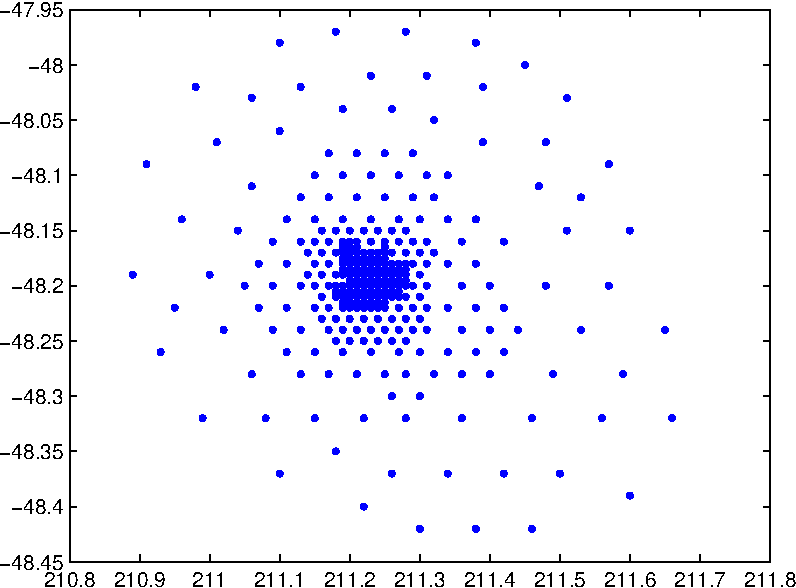
\includegraphics[width=8cm, height=5cm]{./figures/beispiel_scattered_data}
\end{center}
\end{frame}
%
% Slide
% 
\begin{frame}[fragile]\frametitle{Beispiel}
\begin{lstlisting}
>> xi=linspace(min(x),max(x),40);
>> yi=linspace(min(y),max(y),40);
>> [XI,YI]=meshgrid(xi,yi);
>> ZI=griddata(x,y,z,XI,YI,'cubic');
>> surf(XI,YI,ZI)
\end{lstlisting}
\begin{center}
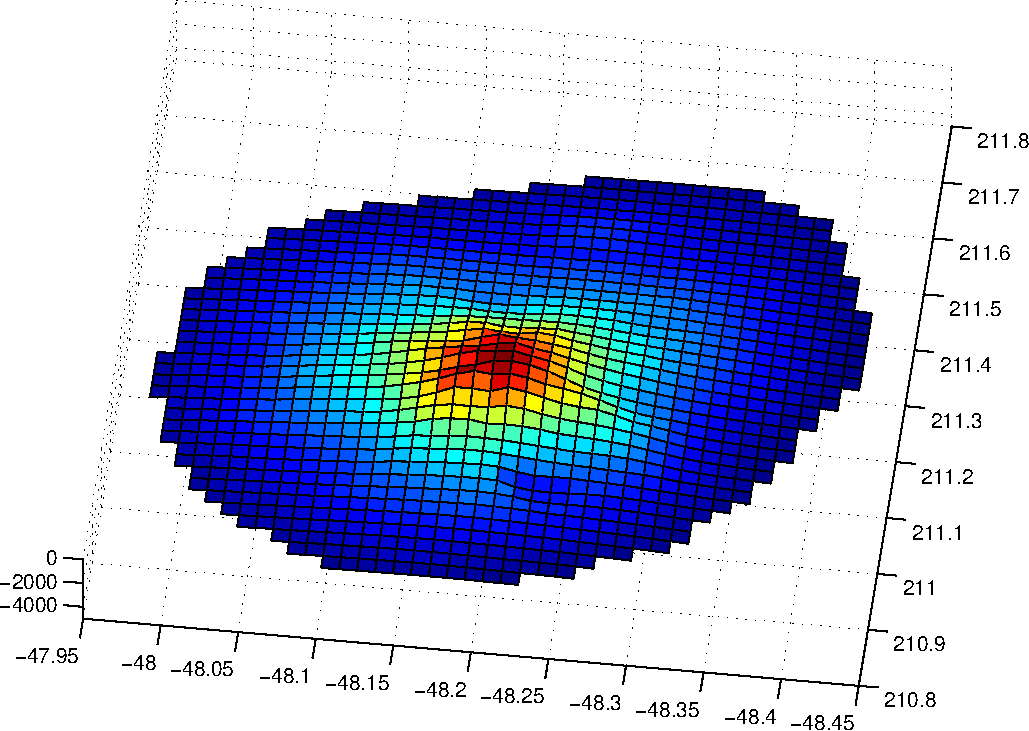
\includegraphics[width=6cm, height=4cm]{./figures/beispiel_scattered_data_plot}
\end{center}
\end{frame}
%
% Slide
% 
\begin{frame}[fragile]\frametitle{griddata}
\begin{lstlisting}
ZI=griddata(x,y,z,XI,YI,methode); 
\end{lstlisting}
\vspace*{-0.5cm}
{\small
\begin{itemize}
\item Vektoren $x,y,z$ enthalten Werte $(x(i),y(i),z(i))$.
\item \lstinline!griddata! interpoliert auf die Stellen $(XI(i,j),YI(i,j))$
  mit Matrizen $XI,YI$. Ergebnis $ZI(i,j)$.
\item Die Art des Interpolierens ist entweder \lstinline!'nearest'!, \lstinline!'linear'!
  oder \lstinline!'cubic'!. Entsprechend wird entweder st\"uckweise konstant, linear
  oder durch bi-kubische Splines interpoliert. 
\item Es wird nur innerhalb der konvexen H\"ulle der Punkte $(x(i),y(i))$
  interpoliert. Ansonsten Funktionswert $NaN$. 
\end{itemize}
}
\end{frame}

%
% Slide
% 
\begin{frame}[fragile]\frametitle{Bemerkungen}
\begin{itemize}
\item Der Interpolation liegt eine Delaunay Triangulation zugrunde. Die Werte
  $(x(i),y(i))$ sind Eckpunkte der entstehenden Dreiecksmenge.
\item Danach werden mit Hilfe der Dreiecke Funktionen  definiert, die
  entsprechende Werte besitzen. 
\item Mittels \lstinline!griddatan! ist die Technik auch auf h\"ohere Dimensionen
  anwendbar. Dreiecke werden durch entsprechende h\"oher-dimensionale
  Simplizes ersetzt. \\
(In 3D Tetraeder)
\end{itemize}
\end{frame}
%
% Slide
% 
\begin{frame}[fragile]\frametitle{interp2}
\begin{lstlisting}
ZI=interp2(X,Y,Z,XI,YI,methode)
\end{lstlisting}
\begin{itemize}
\item Allgemein sind $X,Y,Z$ Matrizen. Dabei ist $Z(i,j)$ der Funktionswert an
  $(X(i,j),Y(i,j))$. $X$ und $Y$ sind in der Regel durch \lstinline!meshgrid! erzeugt. 
\item Es wird an den Stellen $(XI(i,j),YI(i,j))$ interpoliert. Das Ergebnis
  ist $ZI(i,j)$. Die Einträge von $XI$ bzw. $YI$ k\"onnen beliebig sein. 
\item Die Art des Interpolierens ist entweder \lstinline!'nearest'!, \lstinline!'linear'!
  oder \lstinline!'cubic'!. 
%Entsprechend wird entweder st\"uckweise konstant, linear
%  oder durch bikubische Splines interpoliert. 
\end{itemize}
\end{frame}

\part{Tag 4, 2. Teil  \\ Datenstrukturen}
%
%
%
\begin{frame}[fragile]\frametitle{Datenstrukturen}
\begin{itemize}
\item In MATLAB gibt es verschiedene {\it Datentypen}. 
Sie werden bestimmt durch ihre Eigenschaften.
\item Einzelne Elemente eines Datentyps werden {\it Objekte} genannt. 
\item Ein {\it Objekt} besteht meist aus drei Teilen: {\it Bezeichner}, {\it
Referenzen} und {\it Werte} des Objekts.  
\item {\it Variablen} sind Datenobjekte deren Werte w\"ahrend eines
Programmablaufs ver\"andert werden k\"onnen. 
\end{itemize}
\end{frame}
%
%
%
\begin{frame}[fragile]\frametitle{Datentypen in MATLAB}
\begin{itemize}
\item MATLAB speichert alle Variablen als Felder. Ein Skalar ist eine $1 \times
1$-Matrix. 
\item MATLAB weist den Datentyp {\it implizit} zu. Durch die Zuweisung eines
Wertes wird der Typ implizit bestimmt. 
\item Den Datentyp eines Objekts $a$ kann durch den Befehl \alert{
\lstinline!class(a)!} bestimmt werden.
\end{itemize}
\end{frame}
%
%
%
\begin{frame}[fragile]\frametitle{Datentypen in MATLAB}
\begin{itemize}
\item Gleitkommazahlen (Komplexe Zahlen)
\item Characters und Strings
\item Strukturen
\item Cell Arrays
\item Funktionen
\item Sparse Matrizen
\item Integer-Zahlen
\item Logische Ausdr\"ucke
\end{itemize}
\end{frame}
%
% Folie
%
\begin{frame}[fragile]\frametitle{Gleitkommazahlen}
\begin{itemize}
\item Standard-Datentyp ist ein Array von Gleitkommazahlen (\lstinline!double!).
\item Abstand von $1$ zur nächsten Gleitkommazahl in MATLAB: $\epsilon
  =2^{-52}$ (vgl. \lstinline!eps! in MATLAB)
\item Sei $x \in \mathbb{R}$ eine reelle Zahl und $\tilde x$ die
  Darstellung in MATLAB. Dann gilt für den Rundungsfehler \\[-0.5cm]
\[ \frac{|x - \tilde x|}{|x|}\leq \frac{1}{2} \epsilon .\]
\item Die größte bzw. kleinste in MATLAB darstellbare positive Zahl
  ist in
\lstinline!realmin! bzw. \lstinline!realmax! gespeichert. 
\end{itemize}
\end{frame}
%
% Folie
%
\begin{frame}[fragile]\frametitle{Ausnahmen}
\begin{itemize}
\item Ist eine Zahl größer als \lstinline!realmax!, so meldet MATLAB einen
  'Overflow' und gibt als Ergebnis \lstinline!Inf! zurück.
\begin{lstlisting}
>> realmax*1.1
ans =   Inf
\end{lstlisting}
\item Bei Operationen wie $0/0$  oder $\infty / \infty$, erhält man als Ergebnis
  \lstinline!NaN! ({\it Not a Number}).
\begin{lstlisting}
>> 0/0
Warning: Divide by zero.
ans =   NaN
\end{lstlisting}
\end{itemize}
\end{frame}
%
% Folie
%
\begin{frame}[fragile]\frametitle{Umgang mit NaN und       Inf  }
\begin{itemize}
\item Mit Hilfe von \alert{ \lstinline!isinf!} und \alert{ \lstinline!isnan!} kann auf
$\infty$ bzw. NaN getestet werden.
 \begin{lstlisting}
>> isnan(0/0), isinf(1.2*realmax)
ans =   1  ans =   1
\end{lstlisting}
\item Test auf NaN durch $==$ ist nicht m\"oglich
\begin{lstlisting}
>> 0/0 == NaN
ans =     0
\end{lstlisting}
\item Bei Inf ist der Test durch $==$  m\"oglich!
\begin{lstlisting}
>> (1.2*realmax)==Inf
ans =     1
\end{lstlisting}
\end{itemize}
\end{frame}
%
% Folie
%
\begin{frame}[fragile]\frametitle{Single}
\begin{itemize}
\item \"Ahnlich wie in C gibt es den Datentyp \lstinline!single!. Es ist eine
Darstellung in geringerer Genauigkeit. 
\item Durch den Befehl \alert{ \lstinline!single()!} wird eine \lstinline!double!-Zahl in
eine \lstinline!single!-Zahl konvertiert. 
\item Arithmetische Operationen mit \lstinline!double!- und \lstinline!single!-Objekten
ergeben  \lstinline!single!-Objekte.
\end{itemize}
\end{frame}
%
% Folie
%
\begin{frame}[fragile]\frametitle{Single}
\begin{lstlisting}
>> a=sqrt(2); b=single(a);
>> c=a+b; d=a-b
d =
  2.4203e-08
>> whos
  Name   Size     Bytes  Class    
  a      1x1        8  double              
  b      1x1        4  single              
  c      1x1        4  single              
  d      1x1        4  single          
>> [realmax, single(realmax)], realmax
ans =
   Inf   Inf
ans =
  1.7977e+308
\end{lstlisting}
\end{frame}
%
% Folie
%
\begin{frame}[fragile]\frametitle{Operator Rangfolge}
\begin{tabular}{|lp{10cm}|}
%\hline
%Level & Operator\\
\hline
1 &   Exponent (\lstinline!^!, \lstinline!.^!), \lstinline!transpose!\\
2 & logische Verneinung (\lstinline!~!)\\
3 & Multiplikation (*,.*), Division (/,./,\lstinline!\!, \lstinline!.\!)\\
4 & Addition (+), Subtraktion (-)\\
5 & Doppelpunktoperator (:)\\
6 & Vergleichsoperatoren (<,>,<=,>=,==,\lstinline!~=!)\\ 
7 & Logisches und (\lstinline!&!)\\
8 & Logisches oder (|)\\
\hline
\end{tabular}\\
{\tiny Bei gleicher Rangfolge wertet MATLAB von links nach rechts
  aus. \\
Die Rangfolge kann durch Klammersetzung geändert werden.}

\end{frame}
%
% Folie
%
\begin{frame}[fragile]\frametitle{Darstellungsformate am \\ Beispiel $1/7$}
\begin{tabular}{ll}
\alert{ \lstinline!format short!} &  0.1429 \\
\alert{ \lstinline!format short e! }& 1.4286e-01\\
\alert{ \lstinline!format short g! }&0.14286\\
\alert{ \lstinline!format long! }& 0.14285714285714\\
\alert{ \lstinline!format long g! }& 0.142857142857143\\
\alert{ \lstinline!format long e! }& 1.428571428571428e-01\\
\end{tabular}
Das Default-Format ist \lstinline!short!. 
\end{frame}
%
% Folie
%
\begin{frame}[fragile]\frametitle{Komplexe Zahlen}
Komplexe Zahlen $z \in \mathbb{C}$ haben die Form
\[ z = x +iy, \quad x,y \in \mathbb{R} \]
mit $i=\sqrt{-1}$. 
\begin{itemize}
\item $\sqrt{-1}$ ist in MATLAB vordefiniert in den Variablen $i$,$j$.
\item Durch \lstinline!complex(x,y)!  kann aus $x,y \in
  \mathbb{R}$ die komplexe Zahl $x + iy$ erzeugt werden.
\item Für $z=x+iy \in \mathbb{C}$ erhält man den Realteil mit
  $real(z)$ und den Imaginärteil durch $imag(z)$. 
\end{itemize} 
\end{frame}
\begin{frame}[fragile]\frametitle{Polarkoordinaten}
\alert{ \[ z \in \mathbb{C}, \quad z=re^{i \varphi}=r(\cos \varphi + i \sin
  \varphi) \]}
\begin{itemize}
\item \lstinline!abs(z)! ergibt den Betrag $r$ von $z$.
\item $\varphi$ erhält man durch \lstinline!angle(z)!.
\item grafische Darst.:  \lstinline!compass(z)! ($z=3+3i$). \\
 \centering{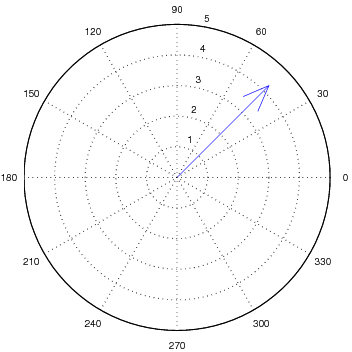
\includegraphics[width=3cm, height=3cm]{./figures/kompass}}\\ 
\end{itemize}
\end{frame}

%
% Folie
%
\begin{frame}[fragile]\frametitle{Structures}
\alert{Structures:}\\
Strukturen sind eine Möglichkeit verschiedene Objekte in einer
Datenstruktur zu bündeln.\\[1cm]

\alert{Beispiel:} komplexe Zahlen
\begin{lstlisting}
>> komp_Zahl.real=1;
>> komp_Zahl.imag=1;
>> komp_Zahl

komp_Zahl = 

    real: 1
    imag: 1
\end{lstlisting}
\end{frame}
%
% Folie
%
\begin{frame}[fragile]\frametitle{Structures II}
\begin{itemize}
\item Alternativ können Strukturen durch
\begin{lstlisting}
struktur = struct('Feld1',Wert1,'Feld2',Wert2,...)
\end{lstlisting}
definiert werden.
\item Ein Feld einer Struktur \lstinline!struktur! kann durch 
\begin{lstlisting}
struc2 = rmfield( struktur ,'Feld')
\end{lstlisting}
gel\"oscht werden. 
\end{itemize}
\end{frame}
%
% Folie
%
\begin{frame}[fragile]\frametitle{Cell Arrays}
\alert{Cell Arrays:} \\
Cell Arrays sind spezielle Matrizen, deren  Einträge aus unterschiedlichen
Datentypen bestehen können. Erzeugt
werden sie durch geschweifte Klammern.\\
\begin{lstlisting}
>> C=\lstinline!{! 1:10, hilb(4);...
       'Hilbert Matrix', pi\lstinline!}!
C = 
       [1x10 double]    [4x4 double]
    'Hilbert Matrix'    [    3.1416]
\end{lstlisting} 
\end{frame}
%
% Folie
%
\begin{frame}[fragile]\frametitle{Befehle für Cell Arrays}
\begin{itemize}
\item Zugriff auf Cell-Arrays:\\ 
\begin{minipage}{5cm}
\begin{lstlisting} 
>> \lstinline!C{2,1}!
ans =
Hilbert Matrix
\end{lstlisting}
\end{minipage}
\begin{minipage}{5cm}
\begin{lstlisting}
>> \lstinline!C{1,2}(2,3)!
ans =
    0.2500
\end{lstlisting}
\end{minipage}
\item Durch \lstinline!celldisp(C)! wird der Inhalt von $C$ dargestellt.
%\item \lstinline!struct2cell! bzw. \lstinline!num2cell! erzeugt ein Cell Array
%  aus einer Struktur bzw. einer normalen Matrix.
\item \lstinline!cellplot(C)! stellt $C$ grafisch dar.
\end{itemize}
\end{frame}
%
% Folie
%
\begin{frame}[fragile]\frametitle{Integer}
\begin{itemize}
\item In diesen Datentypen werden ganze bzw. nat\"urliche Zahlen gepeichert.  
\item Zur effizienten Speicherung gibt es die Datentypen \lstinline!int8!,
\lstinline!uint8!, \lstinline!int16!, \lstinline!uint16!, \lstinline!uint16!, \lstinline!int32!,
\lstinline!uint32!, \lstinline!int64!, \lstinline!uint64!. 
\item In den Datentypen, die mit \lstinline!u! beginnen, werden nat\"urliche Zahlen
gespeichert, sonst ganze Zahlen.
\item Die abschlie{\ss}ende Zahl gibt den Speicherbedarf an. \lstinline!uint8!
ben\"otigt z.B. $8$-Bit. (Wertebereich $0 \dots 2^8-1$).
\end{itemize}
\end{frame}
%
% Folie
%
\begin{frame}[fragile]\frametitle{Integer}
\begin{lstlisting}
>> a=int8(20); b=int16(20); c=int8(20);
>> a*c, a*b
ans =  127
??? Error using ==> mtimes
Integers can only be combined with integers
of the same class, or scalar doubles.
>> a+0.2
ans =   20
>> a+0.5
ans =   21
>> a*1.54
ans =   31
\end{lstlisting}
\end{frame}
%
%
%
\part{Tag 4,  3. Teil  \\ In- und Output}
%
% Slide
%
\begin{frame}[fragile]\frametitle{Input und Output}
\begin{itemize}
\item Benutzereingabe
\item einfache und formatierte Ausgabe
\item Schreiben in Dateien
\item Einlesen von Daten aus Dateien
\item Speichern und Laden von Variablen\\
\item Durch \alert{ \lstinline!help iofun!} erhält man eine Übersicht aller Ein- und
  Ausgabe - Befehle
\end{itemize}
\end{frame}
%
% Slide
%
\begin{frame}[fragile]\frametitle{Benutzereingabe}
\begin{itemize}
\item Standardeingabe: \alert{ \lstinline!input!}
%\item Eingabe eines Zeichens:
\item Informationssteuerung durch die Maus: \alert{ \lstinline!ginput!}
\item Anhalten der Prozedur bis eine Tastatureingabe erfolgt: \alert{
  \lstinline!pause!} 
\end{itemize}
\end{frame} 
%
% Slide
%
\begin{frame}[fragile]\frametitle{input}
Die Benutzereingabe kann durch den Befehl \lstinline!input('Text')! erfolgen. Es
wird der 'Text'  angezeigt. Die Eingabe kann hinter 'Text' erfolgen
und wird durch Return
abgeschlossen.  Durch die Option 's' wird ein String abgefragt.
  
\begin{lstlisting}
>> startwert=input('Bitte geben Sie den Startwert ein: ')
Bitte geben Sie den Startwert ein: 56
 startwert =
     56

\end{lstlisting}
\begin{lstlisting}
>> f=input('Eingabe einer Funktion: ', 's')
Eingabe einer Funktion: sin(x)*cos(x)
f =
sin(x)*cos(x)
\end{lstlisting}
\end{frame}
%
% Slide
%
\begin{frame}[fragile]\frametitle{ginput}
Das Kommando 
\begin{lstlisting}
[x,y]=ginput(n)
\end{lstlisting}
gibt die Vektoren $x$ und $y$ der Koordinaten der nächsten $n$
Maus-Klicks zurück, an denen sich die Maus im aktuellen Grafik-Fenster
befindet.  
\begin{itemize}
\item \lstinline![x,y]=ginput! sammelt so lange Daten ein, bis die
  Return-Taste gedrückt wird.
\item \lstinline![x,y,taste]=ginput(n)! gibt auch den Vektor \lstinline!taste!
  zurück, der aus Werten $1$ (linke Maustaste), $2$ (mittlere
  Maustaste) oder $3$ (rechte Maustaste) besteht. 
\end{itemize} 
\end{frame}
%
% Slide
%
\begin{frame}[fragile]\frametitle{Bezier-Polynom}
\alert{ \[ z (t):=\sum_{i=0}^n {\bf b}_i B_i^n(t), \quad t \in [0,1] \]}
\begin{itemize}
\item $z(t): [0,1] \rightarrow \mathbb{R}^2$ ist das {\it Bezier-Polynom}.
\item ${\bf b}_i \in \mathbb{R}^2$ sind die vorgegebenen 
{\it Kontrollpunkte}.
\item $B_i^n(t)=\left( n \atop i \right) t^i (1-t)^{n-i}$ sind 
{\it Bernstein-Polynome}.
\end{itemize}
\end{frame}
%
% Slide
%
\begin{frame}[fragile]\frametitle{Bezier-Polynom}
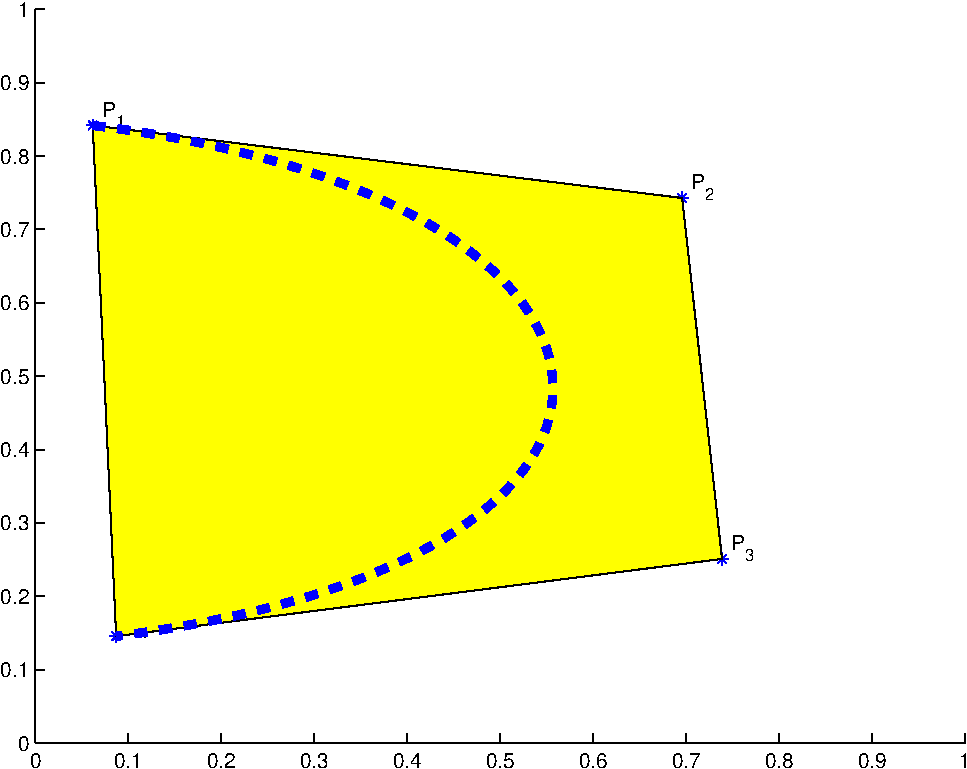
\includegraphics[width=\linewidth,
  height=6.5cm]{./figures/bezier}
\end{frame}
%
% Slide
%
\begin{frame}[fragile]\frametitle{Bezier-Polynom}
\begin{lstlisting}
% Eingabe der 4 Kontrollpunkte
axis([0 1 0 1]); hold on;
for k=1:4
[x(k),y(k)]=ginput(1);
plot(x(k),y(k),'*'); 
text(x(k)+0.01,y(k)+0.01,strcat('P_',num2str(k)));
end;

% Zeichnen der Kontrollpolygons
fill(x,y,'y');

u=0:0.01:1;
umat=[(1-u).^3; 3.*u.*(1-u).^2; 3.*u.^2.*(1-u);u.^3];
plot(x*umat, y*umat,'--','Linewidth',4); hold off;
\end{lstlisting}
\end{frame}
%
% Slide
%
\begin{frame}[fragile]\frametitle{Ausgabe}
\begin{itemize}
\item Angeben einer Variable ohne Semicolon:
\begin{lstlisting}
>> text=['Pi mit 5 signifikanten Stellen : ' num2str(pi,6)]
text =
Pi mit 5 signifikanten Stellen : 3.14159
\end{lstlisting} 
\item Ausgabe des Strings $X$ durch  \lstinline!disp(X)!
\begin{lstlisting}
>> disp(text)
Pi mit 5 signifikanten Stellen : 3.14159
\end{lstlisting} 
\item Ausgabe durch  \lstinline!fprintf()!
\begin{lstlisting}
>> fprintf('Pi mit %1.0f Nachkomma-Stellen : %6.4f \lstinline!\n!',4,pi)
Pi mit 4 Nachkomma-Stellen : 3.1416 
\end{lstlisting}
\end{itemize}
\end{frame}
%
% Slide
%
\begin{frame}[fragile]\frametitle{fprintf- Formartierte Ausgabe}
{\tiny
\begin{lstlisting}
fprintf( Format, Argument1, Argument2,...)
\end{lstlisting}
{\it Format} ist ein String der das genaue Output-Form
der Argumente (Werte der Variablen) bestimmt: 
\begin {bunt}
Format='<*>%<\(\pm\)> <v1.n1><typ1><*>%<\(\pm\)> <v2.n2><typ2><*>...'
\end{lstlisting} 
\begin{itemize}
\item [<*>] Hier kann beliebieger Text eingegeben werden.
\item [<$\pm$>] Durch '+' wird die Angabe des Vorzeichens
  erzwungen. Durch '-' wird eine linksbündige Ausgabe
  erzeugt. Weglassen von <$\pm$> erzeugt eine rechtsbündige Ausgabe
  ohne Anzeige des '+' Zeichens.
\item [vi] Durch $vi$ wird die Anzahl der insgesamt dargestellten Zeichen 
   von Argumenti gesteuert.
\item [ni] Hierdurch wird entsprechend die Anzahl von Nachkommastellen
  angegeben. 
\item [typi] Gibt den Datentyp und Darstellungsformat von Argumenti
  an: \alert{ f} (Standarddarstellung von Gleitkommazahlen), \alert{ e}
  (Expontialdarstellung von Gl.), \alert{ g} (entweder Darst. $f$ oder
  $e$), $s$ (Strings),... 
\end{itemize}
}
\end{frame}
%
% Slide
%
\begin{frame}[fragile]\frametitle{Bemerkungen zu fprintf}
\begin{itemize} 
\item Die formatierte Ausgabe ist an den Ansi-C Standard angelehnt.
\item Durch \lstinline!'\n'! wird ein Zeilenumbruch bewirkt. \lstinline!'\%'! erzeugt
  \lstinline!%!.
 \item \lstinline!sprintf! funktioniert wie \lstinline!fprintf!. Allerdings wird
  die Ausgabe als String zurückgegeben. 
\item Ist ein Argument eine Matrix, so wird fprintf 'vektorisiert'.
\end{itemize}
\end{frame}
%
% Slide
%
\begin{frame}[fragile]\frametitle{Schreiben in Dateien - Beispiel}
\begin{lstlisting}
% waehrung.m
% 
% Erstellt eine Umrechnungstabelle zwischen 
% Euro und anderer Waehrung

waehrung_name=input('Umrechnungstabelle fuer welche Waehrung ? ','s');
fprintf('Ein Euro entspricht wievielen %s ? ',waehrung_name);
umrechnung=input('');
a=[1 2 3 5 10 20 50 100 200 1000];

fid=fopen('umrechnung.txt','w');
fprintf(fid,['Umrechnungstabelle: Euro-',waehrung_name,'\lstinline!\n\n!']);
fprintf(fid,['%7.2f Euro = %7.2f ',waehrung_name,'\lstinline!\n!'],...
  [a;umrechnung*a]);
fprintf(fid,'\lstinline!\n \n! Umrechnungskoeffizient: %3.2f \lstinline!\n!',umrechnung); 
fclose(fid);
\end{lstlisting}
\end{frame}
%
% Slide
%
\begin{frame}[fragile]\frametitle{fopen}
\begin{lstlisting}
fid=fopen(dateiname, erlaubnis)
\end{lstlisting}

\lstinline!fopen! öffnet die Datei \lstinline!dateiname! im Modus
  \lstinline!erlaubnis! und erzeugt einen
  Datei-Handle \lstinline!fid!. Für \lstinline!erlaubnis! gibt es u.a. die folgenden
  Möglichkeiten:
{%\tiny 
\begin{itemize}
\item ['r']  Lesen aus der Datei.
\item ['w']  Schreiben in die Datei (Erzeugen falls nötig)
\item ['a']  Hinzufügen (Erzeugen falls nötig)
\item ['r+'] Lesen und schreiben (aber nicht erzeugen) 
\end{itemize}
}
\end{frame}
%
% Slide
%
\begin{frame}[fragile]\frametitle{Weitere Kommandos}
\begin{itemize}
\item \lstinline!fclose(fid)! schliesst die Datei mit dem Handle \lstinline!fid!
\item Mit dem Befehl
\begin{lstlisting}
fprintf( Datei-Handle, Format, Argument1, Argument2,...)
\end{lstlisting}
wird in die durch das Datei-Handle angegebene Datei gemäß der obigen
Konventionen geschrieben.
\item Durch ein  zusätzliches Output-Argument können Fehler aufgefangen
  werden. 
\begin{lstlisting}
[fid, message]=fopen(dateiname, erlaubnis)
\end{lstlisting}
Ist  die Datei nicht zu öffnen, so ist \lstinline!fid=-1!. 
\end{itemize}
\end{frame}
%
% Slide
%
\begin{frame}[fragile]\frametitle{Lesen aus einer Datei}
\begin{lstlisting}
% waehrung_auslesen.m
% 
% Liest eine Umrechnungstabelle aus der
% Datei 'umrechnung.txt'

clear all;
fid=fopen('umrechnung.txt','r');
waehrung_name=fscanf(fid,'Umrechnungstabelle: Euro-%s');
daten=fscanf(fid,['%f Euro = %f ',waehrung_name],[2 inf]);
umrechnung=fscanf(fid,'Umrechnungskoeffizient: %f'); 
fclose(fid);
  
% Ausgabe
fprintf('Umrechnung: Euro - %s: Kurs: %f \lstinline!\n!',...
    waehrung_name,umrechnung);
fprintf(' %7.2f Euro  = %7.2f  \lstinline!\n!',daten);
\end{lstlisting}
\end{frame}
%
% Slide
%
\begin{frame}[fragile]\frametitle{fscanf}
\begin{lstlisting}
[daten,anz]=fscanf(fid,format,Größe)
\end{lstlisting}
\begin{itemize}
\item \lstinline!fscanf! liest Daten aus der Datei mit dem Handle
  \lstinline!fid!. 
\item Die Daten werden in \lstinline!daten! gespeichert. Der optionale Wert
  \lstinline!anz! gibt die Anzahl erfolgreich gelesener Daten an.
\item \lstinline!format! gibt das vorgegebene Suchmuster vor.
\item Die \lstinline!Größe! gibt die Dimension der Output-Matrix an.
\end{itemize}
\end{frame}
%
% Slide
%
\begin{frame}[fragile]\frametitle{Weitere Befehle}
\begin{itemize}
\item Der Befehl \alert{ \lstinline!fgetl(fid)!} liest eine Zeile aus der Datei mit
  Handle \lstinline!fid! und gibt die Zeile als String zurück.
\item Ob das Dateiende erreicht ist, kann durch den Befehl \alert{
  \lstinline!feof(fid)!} geprüft werden. \lstinline!feof(fid)! gibt eine $1$
  zurück, falls das Dateiende erreicht ist und $0$ sonst. 
\end{itemize}
\end{frame}
%
% Slide
%
\begin{frame}[fragile]\frametitle{Beispiel - Bubblesort}
\vspace*{-0.5cm}
\begin{itemize}
\item Bubblesort durchläuft die Datenmenge von Anfang bis zum Ende und
vergleicht paarweise die nebeneinanderstehenden Elemente. 
\item Sind zwei
benachbarte Elemente nicht in der richtigen Reihenfolge, so werden sie
miteinander vertauscht. 
\item Ist man am Ende angekommen, beginnt man wieder
von vorne. 
\item Die Datenmenge ist sortiert, falls bei einem Durchlauf
keine Vertauschungen mehr vorgenommen werden.
\end{itemize} 
\end{frame}
%
% Slide
%
\begin{frame}[fragile]\frametitle{Beispiel - Bubblesort}
\begin{lstlisting}
 function sortieren(dateiname1, dateiname2)
% sortieren   Die Datei dateiname1 wird alphabetisch sortiert
%             und als dateiname2 abgespeichert.
%   INPUT:    STRING dateiname1
%             STRING dateiname2
 
% Datei laden
[fid,message]=fopen(dateiname1,'r');
if fid==-1 
    error('Datei nicht gefunden');
end;
% Datei lesen
anz=0;
while feof(fid)==0
    anz=anz+1;     
    inhalt\lstinline!{anz}!=fgetl(fid); 
end
fclose(fid);
\end{lstlisting}
\end{frame}
%
% Slide
%
\begin{frame}[fragile]\frametitle{Beispiel - Bubblesort (Forts.)}
\begin{lstlisting}
% Sortieren
sortierungen=1; 
while sortierungen>0
    sortierungen=0;
    for k=1:anz-1
        % vergleich_gr(a,b) ist 1 fuer a<b, 0 sonst
        if vergleich_gr(inhalt\verb${k+1}$,inhalt\lstinline!{k}!)
            hilf=inhalt\lstinline!{k}!; inhalt\lstinline!{k}!=inhalt\verb${k+1}$; inhalt\verb${k+1}$=hilf;
            sortierungen=sortierungen+1;
        end
    end
end
% Datei schreiben
fid=fopen(dateiname2,'w');
for k=1:anz
   fprintf(fid,'%s \lstinline!\n!',inhalt\lstinline!{k}!); 
end;
fclose(fid);
\end{lstlisting}
\end{frame}
%
% Slide
%
\begin{frame}[fragile]\frametitle{Bemerkungen}
\begin{itemize}
\item Es ist auch möglich temporäre Dateien zu erzeugen.
\item Binäre Dateien können erzeugt und gelesen werden mit Hilfe der
  Befehle \lstinline!fread! und \lstinline!fwrite!. 
\item  Mittels \lstinline!xlsread! können Excel-Tabellen eingeladen werden.
\item Bilddateien werden durch \lstinline!imread! importiert.
\item  Audiodateien (.wav) bzw. Videodateien (.avi) können durch
  \lstinline!wavread! bzw. \lstinline!aviread! importiert werden. 
\end{itemize}
\end{frame}
%
% Slide
%
\begin{frame}[fragile]\frametitle{Beispiel: Bin\"are Daten}
\begin{lstlisting}
%-------------------- beispiel_bin_data.m
A = hilb(10);

% Schreibe binaere Datei
fwriteid = fopen('hilb10.bin','w');
count = fwrite(fwriteid,A,'double');
fclose =(fwriteid);

% Lesen binaere Datei
freadid = fopen('hilb10.bin','r');
B = fread(freadid, count, 'double');
C = reshape(B,10,10);

disp(norm(A - C))
\end{lstlisting}
\end{frame}
%
% Slide
%
\begin{frame}[fragile]\frametitle{Laden und Speichern von \newline Variablen}
\begin{itemize}
\item \alert{ \lstinline!save filename!} speichert den gesamten
  Workspace in der Datei \lstinline!filename.mat!. Einladen des Workspace
  ist möglich mittels  \alert{ \lstinline!load filename!}. 
\item Mittels \alert{ \lstinline!save filename A x!} werden nur die
  Variablen $A$ und $x$ in der Datei \lstinline!filename.mat!
  gespeichert. Durch  \alert{ \lstinline!load filename!} werden nun die
  Variablen $A$ und $x$ dem Workspace hinzugefügt. 
\item Bei \lstinline!load! werden bestehende Variablen mit dem gleichen
  Namen überschrieben.
\end{itemize}
\end{frame}

\part{Fehler}
%
% Slide
%
\begin{frame}[fragile]\frametitle{Fehler}
% In MATLAB gibt es zwei Arten von Fehler.
\begin{itemize}
\item \alert\alert{ Syntax Fehler}: z.B. Schreibfehler oder
  Weglassen von Klammern. MATLAB entdeckt die meisten Syntax Fehler
  und gibt eine entsprechende Fehlermeldung zurück mit Angabe der
  Zeile. 
\item \alert\alert{ Run-time Fehler}: Diese Fehler sind
  normalerweise algorithmischer Natur. Oft passen z.B. bei
  Matrixoperationen die Matrizen nicht zusammen. \vspace*{-0.5cm}
\end{itemize}
{\tiny Die erste Fehlermeldung zeigt bei geschachtelten Funktionsaufrufen
an, in welcher Funktion der Fehler liegt.}
\end{frame}
%
% Slide
%
\begin{frame}[fragile]\frametitle{Fehler abfangen}
\begin{itemize}
\item Der Befehl \alert{ \lstinline!error('text')!} erzeugt die
  Fehlermeldung \lstinline!text! und bricht das Programm ab. Insebsondere
  die Eingabeparameter sollten auf Fehler geprüft werden.
\item Warnungen werden durch \alert{ \lstinline!warning('text')!} erzeugt. Im
  Gegensatz zu \lstinline!error! wird das Programm aber fortgesetzt. 
\end{itemize}
\end{frame}
%
% Slide
%
\begin{frame}[fragile]\frametitle{Beispiel}
\begin{lstlisting}
function interpolation(f1,N)
\end{lstlisting}
\alert{ \centering{$\cdots$}}\\
\begin{lstlisting}
%----------------- Fehlerbehandlung
if (round(abs(N)) ~= N) | (N==0)
    error(strcat('Bitte fuer die Anzahl der Stuetzstellen',...
    'eine natuerliche Zahl verwenden'));
end
if ~ischar(f1)
    error('Bitte fuer die Funktion einen String verwenden');
end
\end{lstlisting}
\alert{ \centering{$\cdots$}}\\
\end{frame}

